\documentclass[border=0.8ex,svgnames,tikz]{standalone}
\usepackage{amsmath,mathtools}
\usepackage{fontspec}
\setmainfont{Source Serif 4}
\setsansfont{Source Sans 3}
\setmonofont{Source Code Pro}
\begin{document}
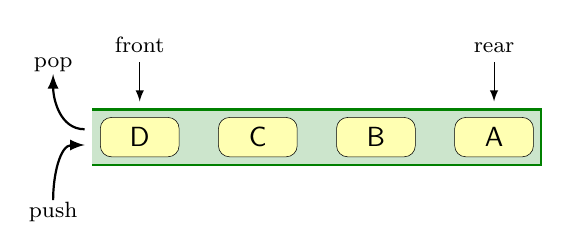
\begin{tikzpicture}[
  queue element/.style={
    draw,
    very thin,
    rounded corners,
    fill=Yellow!30,
    minimum width=1cm,
    minimum height=.5cm,
    font=\sffamily,
  },
  >=latex,
  ]
  \path[fill=Green!20] (5.1,.35) rectangle (-.6,-.35);
  \path[draw=Green,thick] (-.6,.35) -- (5.1,.35) |- (-.6,-.35);
  \foreach \i/\name in {0/D,1/C,2/B,3/A} {
    \node[queue element] (\name) at (1.5*\i,0) {\name};
  };
  \path[draw,<-] ([yshift=.2cm]A.north) -- ++(0,.5)
  node[above,font=\footnotesize]{rear};
  \path[draw,<-] ([yshift=.2cm]D.north) -- ++(0,.5)
  node[above,font=\footnotesize]{front};
  \path[draw,->,thick] (-.7,+.1) to[out=180,in=270] ++(-.4,+.7)
  node[above,font=\footnotesize,inner sep=0.1ex]{pop};
  \path[draw,->,thick] (-.7,-.1) ++(-.4,-.7)
  node[below,font=\footnotesize,inner sep=0.1ex]{push} to[out=90,in=180] (-.7,-.1);
\end{tikzpicture}
\end{document}
